\documentclass[a4paper]{article}

\usepackage{paracol} % allows multiple columns
\usepackage{eso-pic} % creates the gray rectangle in the background
\usepackage{xcolor} % allows color picking
\usepackage{tikz} % creates the rectangle aroung the name+profession
\usepackage{fontspec} % allows changing fonts settings
\usepackage{anyfontsize} % allows selection of different font sizes
\usepackage{fix-cm}
\usepackage{setspace} % changes space between lines
\usepackage[showframe]{geometry} % shows the page layout
%\usepackage{layout} % shows the page layout and dimensions of the layout as an image
% \usepackage{geometry} % changes page layout
\usepackage{changepage} % changes column width

\usepackage[english]{babel} % correctly and automatically hyphenate english words
\usepackage{lipsum}

\backgroundcolor{c[0]}[rgb]{1,0.8,1} % visualize left  column
\backgroundcolor{c[1]}[rgb]{1,1,0.8} % visualize right column

\geometry{
	total={210mm,297mm}, 	% set A4 size
	left=0.62in,				% make margins equal in every side
	right=0.62in,				% make margins equal in every side
	top=0.42in,				% make margins equal in every side
	bottom=1in,				% make margins equal in every side
	marginparwidth=0in,		% remove margin notes
	marginparsep=0in,		% remove margin notes
	headheight=0in,			% remove header
	headsep=0in,			% remove header
	footskip=0in			%remove footer
}

% sets the gray rectangle as background
\AddToShipoutPictureBG{\color[RGB]{244,244,244}%
	\AtPageLowerLeft{\rule{2.57in}{\paperheight}}} % this lines defines the rectangle position (lower left) and sizes(width = 2.57 inches, height = current paperheight (297mm))

\newfontfamily{\mtstitle}[LetterSpace=10]{Montserrat} % creates a new font family with more spacing for the title
\newfontfamily{\mtsl}[UprightFont={* Light}]{Montserrat} % creates a new font family for the light version of Montserrat

\pagenumbering{gobble} % disables page numbering

\begin{document}
	% HACK: the line below is a hack that affects the spacing between every float and the underlying text. Shouldn't be a problem since this is the only float we're going to use.
	% \setlength{\intextsep}{0.44in plus 2.0pt minus 2.0pt} % changes spacing between title and text
	% creates the rectangle that contains the name and profession
	\begin{figure}[!ht]
		\centering
		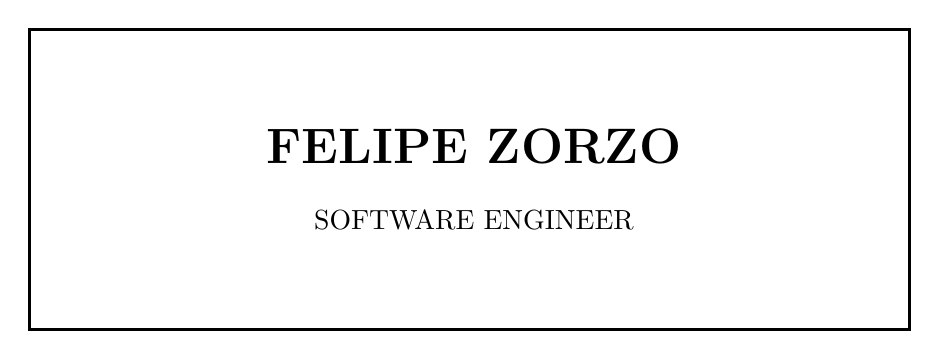
\begin{tikzpicture}
			\node[rectangle, draw, fill=white, very thick, align=center, font=\setstretch{2}, minimum width = 4.4in, minimum height = 1.5in] (r) at (0,0)
			{%
				{\mtstitle \fontsize{18}{21.6} \textbf{FELIPE ZORZO}}\\%
				{\mtsl \fontsize{10}{12} SOFTWARE ENGINEER}%
			};
		\end{tikzpicture}
	\end{figure}

	\begin{paracol}{2}
		\fontspec{Montserrat}

		\begin{column}
			\fontsize{7}{8.4}\selectfont
       		\begin{adjustwidth}{0in}{1.82in}
				\sloppy
				Ggray
				\lipsum
        	\end{adjustwidth}
		\end{column}

		\begin{column}
			\begin{adjustwidth}{-1.37in}{0in}
				\sloppy
				Ggray
				\lipsum
			\end{adjustwidth}
		\end{column}

	\end{paracol}
%	\newpage
%	\layout* % shows the page layout and its dimensions
\end{document}